Podemos fácilmente procesar las consultas de sumas en un arreglo estático construyendo un arreglo de suma en prefijos(prefix sum). Donde cada valor en el prefix array es igual a la suma en el arreglo original hasta esa posición. Por ejemplo tenemos que el valor en la posicion k es la función $sum_{q}(0,k)$.

Este prefix sum array puede ser construido en una complejidad $O(n)$.

Consideremos el siguiente ejemplo:

$\begin{array}{ccccccccc}
 \textbf{Indice}	& 0 &  1 & 2 & 3 & 4 & 5 & 6 & 7 \\ 
	\textbf{ Valor} & 1	& 3 & 4 & 8 & 6 & 1 & 4 & 2 
\end{array} $

La suma de prefijo correspondiente al arreglo anterior es:

$\begin{array}{ccccccccc}
	\textbf{Indice}	& 0&  1 & 2 & 3 & 4 & 5 & 6 & 7 \\ 
   \textbf{ Valor} &	1	& 4 & 8 & 16 & 22 & 23 & 27 & 29 
\end{array}$ 

Ahora como el prefix sum array contiene todos los valores de $sum_{q}(0,k)$, entonces podemos calcular todos los valores de $sum_{q}(a,b)$ en tiempo $O(1)$ de la manera siguiente:

$ sum_{q}(a,b)= sum_{q}(0,b) - sum_{q}(0,a-1) $


A continuación veamos un ejemplo de como funcionan estas consultas. Consideremos que queremos obtener la suma en el rango $[3,6]$.

$\begin{array}{ccccccccc}
\textbf{Indice}	&	0&  1 & 2 & 3 & 4 & 5 & 6 & 7 \\ 
\textbf{ Valor} & 1	& 3 & 4 & \textcolor{red}{8} & \textcolor{red}{6} & \textcolor{red}{1} & \textcolor{red}{4} & 2 
\end{array} $

En este caso $ sum_{q} (3,6) = 8 + 6 + 1 + 4 = 19$. Esta suma puede ser calculada utilizando los dos valores del prefix sum array señalados.

$\begin{array}{ccccccccc}
\textbf{Indice}	&	0&  1 & 2 & 3 & 4 & 5 & 6 & 7 \\ 
\textbf{ Valor} &	1	& 4 & \textcolor{red}{8} & 16 & 22 & 23 & \textcolor{red}{27} & 29 
\end{array} $

Entonces, $sum_{q}(3,6) = sum_{q}(0,6)-sum_{q}(0,2)=27-8=19$.

\subsection{Suma de prefijos en dos dimensiones}

Tambien podemos generalizar la idea anterior para poder computar en más dimensiones. Por ejemplo podemos construir un prefix sum bidimensional que puede ser usado para calcular la suma de cualquier subarreglo rectangular en tiempo $O(1)$. Donde cada suma en tal arreglo corresponde al subarreglo que comienza en la esquina superior izquierda de la matriz y termina en la posicion de la matriz a donde accedemos.

El siguiente esquema ilustra la idea anterior:

% TODO: \usepackage{graphicx} required
\begin{figure}[h!]
	\centering
	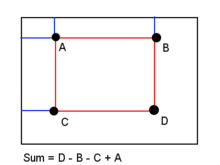
\includegraphics[width=0.2\linewidth]{img/prefix_sum_2D}
	\label{fig:prefixsum2d}
\end{figure}

La suma de prefijo se puede calcular de manera eficiente en un solo paso sobre la matriz, ya que el valor en el prefijo de suma en $(i,j)$ es simplemente: 

$$PS(i,j) = m(i,j) + PS(i,j-1) + PS(i-1,j) - PS(i-1,j-1)$$

Siendo $SP$ el prefijo de suma , $m$ la matriz con los valores originales y $i$ , $j$ indican una posición dentro de la matriz. Se bebe tener en cuenta que la matriz de suma de prefijo se calcula desde la esquina superior izquierda.

Una vez que se ha calculado la matriz de suma de prefijo , la evaluación de la suma sobre cualquier área rectangular requiere exactamente cuatro referencias de matriz, independientemente del tamaño del área. Es decir, tiene $A = (i_0 , j_0)$ , $B = ( i_1 , j_0 )$ , $C = ( i_0 , j_1 )$ y $D = ( i_1 , j_1 )$ , la suma de $p(i,j)$ sobre el rectángulo formado por $A , B , C$ y $D$ es:

$$ \sum_{ i_0 < i \le i_1 \quad j_0 < j \le j_1}^{} p(i,j) = PS(D)+PS(A)-PS(B)-PS(C) $$

La siguientes gráficas ilustran mejor la idea:

% TODO: \usepackage{graphicx} required
\begin{figure}[h!]
	\centering
	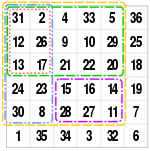
\includegraphics[width=0.35\linewidth]{img/prefix_sum_2D_a}
	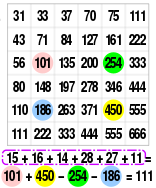
\includegraphics[width=0.35\linewidth]{img/prefix_sum_2D_b}
	\label{fig:prefixsum2da}
\end{figure}
